% https://tex.stackexchange.com/questions/742061/how-to-encapsulate-this-interface-or-make-some-recursion-design-in-this-graph-th
\documentclass[tikz,border=8pt]{standalone}
\usetikzlibrary{shapes.geometric,calc}
\pgfmathsetseed{4321}
\tikzset{line cap=round,line join=round}
\begin{document}
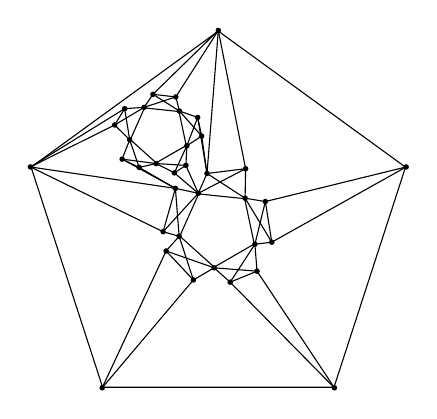
\begin{tikzpicture}
    \node[name=O1,regular polygon, regular polygon sides=5, draw,minimum size=5cm,inner sep=5pt] {};
    \foreach \i in {1,...,5}{\fill (O1.corner \i) circle (1pt);}
    \node[name=O2,regular polygon, regular polygon sides=5, draw,minimum size=1cm,inner sep=5pt,rotate=30] {};
    \foreach \i[evaluate = \i as \j using {int(mod(\i,5)+1)}] in {1,...,5}{%
    \fill (O2.corner \i) circle (1pt);
    \pgfmathsetmacro\rndlena{(rnd*30+85)/100}
    \pgfmathsetmacro\rndlenb{(rnd*30+85)/100}
    \pgfmathsetmacro\rndanga{-(15+rnd*20)}
    \pgfmathsetmacro\rndangb{(15+rnd*20)}
    % \node at (rand,rand) {(\rndlen,\rndanga,\rndangb)};
    \coordinate (O2-corner \i\j) at ($(O2.corner \i)!\rndlena!\rndanga:(O2.corner \j)$);
    \fill (O2-corner \i\j) circle (1pt);
    \coordinate (O2-corner \j\i) at ($(O2.corner \j)!\rndlenb!\rndangb:(O2.corner \i)$);
    \fill (O2-corner \j\i) circle (1pt);
    \path (O2-corner \j\i) edge (O2-corner \i\j)
        (O2-corner \j\i) edge (O2.corner \i)
        (O2-corner \j\i) edge (O2.corner \j)
        (O2-corner \i\j) edge (O2.corner \i)
        (O2-corner \i\j) edge (O2.corner \j)
        (O1.corner \j) edge (O2-corner \j\i) edge (O2-corner \i\j) 
        ;
    }
    \begin{scope}
        \node[name=O3,regular polygon, regular polygon sides=5, draw,minimum size=.75cm,inner sep=0pt,rotate=30] at (-.75,1.2) {};
        \foreach \i/\p[evaluate = \i as \j using {int(mod(\i,5)+1)}] in%
        {%
            1/{O1.corner 2},
            2/{O2-corner 21},
            3/{O2.corner 1},
            4/{O2-corner 51},
            5/{O1.corner 1}%
        }
        {%
        \pgfmathsetmacro\rndlena{(rnd*20+40)/100}
        \pgfmathsetmacro\rndlenb{(rnd*20+40)/100}
        \pgfmathsetmacro\rndanga{-(50+rnd*30)}
        \pgfmathsetmacro\rndangb{(50+rnd*30)}
        % \node at (rand,rand) {(\rndlen,\rndanga,\rndangb)};
        \fill (O3.corner \i) circle (1pt);
        \coordinate (O3-corner \i\j) at ($(O3.corner \i)!\rndlena!\rndanga:(O3.corner \j)$);
        \fill (O3-corner \i\j) circle (1pt);
        \coordinate (O3-corner \j\i) at ($(O3.corner \j)!\rndlenb!\rndangb:(O3.corner \i)$);
        \fill (O3-corner \j\i) circle (1pt);
        \path (O3-corner \j\i) edge (O3-corner \i\j)
            (O3-corner \j\i) edge (O3.corner \i)
            (O3-corner \j\i) edge (O3.corner \j)
            (O3-corner \i\j) edge (O3.corner \i)
            (O3-corner \i\j) edge (O3.corner \j)
            %% a bit dummy here
            (\p) edge (O3-corner \j\i) edge (O3-corner \i\j) 
            ;
        }
    \end{scope}
\end{tikzpicture}
\end{document}